\chapter{Empirical Comparison\label{cha:chapter6}}

This chapter makes use of the tools and concepts investigated in Chapters \ref{cha:approach}, \ref{cha:designing}, \ref{cha:crayon} to perform an empirical comparison of forecasting methods. Specifically, the tuning and benchmarking capabilities of Crayon are used to enable fair, accurate and reproducible comparisons. The forecasting models compared in this Section are those available in GluonTS as of March 18th 2021.


\section{Methodology}
In order to benchmark the forecasting models in GluonTS, Docker images containing GluonTS have to be built. For this the official dockerfiles available in GluonTS are used.  After the images are built, methods of speeding up backtesting are investigated. This is done since several thousands of training jobs are required to run, thus, minimizing the time to backtest saves days of training time. Three different methods of speedup are investigated; GPU acceleration, multiprocessing on CPU and using ultraJSON (ujson) package for serializing and deserializing JSON data. The ujson package is used by GluonTS if installed but is not required as the JSON package from the Python standard library is used by default \cite{gluonts-github}.

After identifying a fast performing configuration the algorithms to benchmark are identified. Due to the size of the comparison, and since the time required to tune and benchmark models differ, a priority list is followed. As the focus of the comparison is on DL based forecasting, those methods utilizing DNNs, CNNs or RNNs have the highest priority. Second highest priority are for recent forecasting models not based on DL. Thereafter, naive methods are chosen as these are quick to evaluate and serve as a good baseline to compare to. After the naive models, classical models such as arima are chosen since these only serve as a source of comparison but are not the focal point of this thesis.

When the models to benchmark are identified, these are tuned to the four datasets chosen in Chapter \ref{cha:designing} using the grid-search functionality in Crayon. The hyperparameter search space is limited for this comparison as several models are to be tuned within a few months on a single machine. Thus in order to ensure that the algorithms are optimally tuned, no limit will be put on the amount of time taken for tuning the algorithms. However, the maximum number of configurations in the grid is set to 300 and the maximum number of different values tested for a single hyperparameter was set to maximum 3. These two limits are imposed as they introduce limits for both models with few hyperparameters and models with multiple hyperparameters as discussed in Section \cite{dockerhub_arangatang}. Furthermore, hyperparameters used for all forecasting models in GluonTS share were tuned in the same way for all models for consistency.

Certain information such as the cardinality of a dataset, the prediction length and the frequency of the data are provided as metadata by the datasets in GluonTS. These values are used when performing the tuning and benchmarking for this comparison.

When using the Grid Search functionality in Crayon, runtool configurations for each tuning job is stored. When the grid-search has finished the configs of the best hyperparameter configurations are then combined into a single Runtool config file. This file is then passed to the Crayon benchmarking system so that the algorithms can be benchmarked using the optimal hyperparameters for each dataset. The BRF generated by the benchmarks are then uploaded to the public GitHub repository of the masterthesis \cite{}.

The specification of the computer used to backtest the different models and relevant software used is presented in Table \ref{tab:sys_spec}.

\begin{table}[htb]
    \centering
    \begin{tabular}{cc}
        \hline
        Component Name     & Component Used                           \\[0.5ex]
        \hline
        CPU                & I7-9700K up to 4.9 GHz                   \\
        GPU                & Nvidia Titan RTX                         \\
        CUDA Version       & 11.2                                     \\
        GPU Driver Version & 460.73.01                                \\
        RAM                & 32 GB DDR4, 3600 MHz                     \\
        Operating System   & Ubuntu 20.04.2                           \\
        Docker Version     & 20.10.6                                  \\
        GluonTS commit     & 4d1a9a09048b1e0db93de885e9636e4add8f91c6 \\
    \end{tabular}
    \caption{Specification of hardware and software used to perform the benchmarks.}
    \label{tab:sys_spec}
\end{table}

\section{Scope and limitations}
To limit the scope of this investigation, only algorithms available in GluonTS were used. Further, only a subset of these could be used due to the time limit of the thesis. As discussed in Section \ref{cha:approach} fair comparisons of advanced algorithms can only be done if the implementations being evaluated are well implemented. Since the algorithms implemented in GluonTS are implemented and used by experienced practitioners in the field of forecasting these algorithms are considered to fulfill this criteria. Only algorithms available in GluonTS up until commit: \textit{4d1a9a09048b1e0db93de885e9636e4add8f91c6} are used for the comparison, any algorithms added at a later time are not considered \cite{gluonts-github}.

Due to the limited time of the thesis in comparison to the number of algorithms which should be compared, not all algorithms in GluonTS can be tuned and benchmarked in time. Further, multivariate algorithms are not compared since GluonTS does not offer any multivariate datasets. Further only three multivariate models are available in GluonTS, GPVar, GPVar and LSTNet. Any comparisons made with these when executed on the datasets identified in \ref{sec:dataset_analysis} would be unfair since only univariate data would be used to train them.

\section{Result}
The initial task of optimizing the Docker images such that they perform well took considerably longer than anticipated. Particularly the use of GPU acceleration was problematic since certain forecasting models such as the \textit{MQCNNEstimator} failed to converge when training. Advice posted on the GluonTS Github page suggested that this issue could be resolved by lowering the learning rate, despite this the issue remained \cite{gluonts-github}. Due to the increased instability, GPU acceleration was deemed unsuitable for the comparison.

The use of the Python package \textit{ujson} showed significant speedup and no negative effects were noticed. Thus, \textit{ujson} is added to the Docker images used for benchmarking and tuning.

Initially, the multiprocessing support when using GluonTS within a Docker image was limited. This caused backtesting to fail sporadically. The underlying cause for this was investigated and a pull request solving this was opened \cite{fix_dockerfile_pr}. While this made multiprocessing stable, the number of threads used could only be controlled up to 4, if more threads vere requested than four it had no effect as the CPU utilization remained the same. However, executing the models on four cores instead of one did improve throughput significantly and was thus utilized for the benchmarks.

Most of the algorithms in GluonTS can be executed through the same Docker image. However, the naive forecasting algorithms, the Prophet forecaster, and the classical models had additional dependencies. Thus in total four Docker images were built. These images are available on the \textit{arangatang/masterthesis} repository on Dockerhub \cite{dockerhub_arangatang}.

Of the 20 algorithms presented in Section \ref{algorithms} four does not require tuning; Prophet, Naive Seasonal, Naive 2 and the Theta from the RForecastPredictor. Since multivariate algorithms are excluded from the study, the GPVAREstimator, DeepVAREstimator and the LSTNET estimators are not tuned. In order to tune the remaining 13 models, 920+ configurations were executed on 4 datasets with 3 repetitions per hyperparameter configuration. Thus, more than 11000 training jobs were executed over the course of four months. An overview of the results from the tuning is presented in Table \ref{tab:tuning_results}.

\begin{table}[htb]
    \centering
    \begin{tabular}{cccccc}
        Algorithm         & \rothalf{Electricity} & \rothalf{Solar Energy} & \rothalf{M4 Daily}   & \rothalf{M5}         & \rothalf{Electricity (GPU)} \\
        \hline
        DeepAR            & \cellcolor{green}X    & \cellcolor{green}X     & \cellcolor{green}X   & \cellcolor{green}X   & \cellcolor{green}X          \\
        DeepFactor        & \cellcolor{green}X    & \cellcolor{green}X     & \cellcolor{green}X   & \cellcolor{green}X   & \cellcolor{green}X          \\
        CanonicalRNN      & \cellcolor{green}X    & \cellcolor{green}X     & \cellcolor{green}X   & \cellcolor{green}X   & \cellcolor{green}X          \\
        SimpleFeedForward & \cellcolor{green}X    & \cellcolor{green}X     & \cellcolor{green}X   & \cellcolor{green}X   & \cellcolor{green}X          \\
        NBEATS Ensamble   & \cellcolor{green}X    & \cellcolor{green}X     & \cellcolor{green}X   & \cellcolor{green}X   & \cellcolor{green}X          \\
        Gaussian Process  & \cellcolor{green}X    & \cellcolor{green}X     & \cellcolor{green}X   & \cellcolor{red} F    & \cellcolor{green}X          \\
        MQCNN             & \cellcolor{green}X    & \cellcolor{green}X     & \cellcolor{green}X   & \cellcolor{green}X   & \cellcolor{red} F           \\
        MQRNN             & \cellcolor{green}X    & \cellcolor{green}X     & \cellcolor{green}X   & \cellcolor{green}X   & \cellcolor{green}X          \\
        Transformer       & \cellcolor{green}X    & \cellcolor{green}X     & \cellcolor{green}X   & \cellcolor{green}X   & \cellcolor{green}X          \\
        DeepState         & \cellcolor{orange}M   & -                      & -                    & -                    & \cellcolor{orange}M         \\
        WaveNet           & \cellcolor{red}F      & -                      & -                    & -                    & \cellcolor{red}F            \\
        NPTS              & \cellcolor{red}F      & -                      & -                    & -                    & \cellcolor{red}F            \\
        Seq2Seq           & -                     & -                      & -                    & \cellcolor{red}F     & -                           \\
        Prophet           & \cellcolor{blue!25}U  & \cellcolor{blue!25}U   & \cellcolor{blue!25}U & \cellcolor{blue!25}U & \cellcolor{blue!25}U        \\
        Naive Seasonal    & \cellcolor{blue!25}U  & \cellcolor{blue!25}U   & \cellcolor{blue!25}U & \cellcolor{blue!25}U & \cellcolor{blue!25}U        \\
        Naive2            & \cellcolor{blue!25}U  & \cellcolor{blue!25}U   & \cellcolor{blue!25}U & \cellcolor{blue!25}U & \cellcolor{blue!25}U        \\
        Theta             & \cellcolor{blue!25}U  & \cellcolor{blue!25}U   & \cellcolor{blue!25}U & \cellcolor{blue!25}U & \cellcolor{blue!25}U        \\
        \hline
    \end{tabular}
    \caption{Tuning results of 16 forecasting algorithms in GluonTS. Legend: X (green) finished successfully, M (orange) memory leak, F (red) failed, U (blue) tuning not required.}
    \label{tab:tuning_results}
\end{table}

Of the 13 models which required tuning, 7 were tuned without major issues, however for five of the algorithms; Gaussian Process (GP), DeepState, WaveNet, NPTS and Seq2Seq harder issues arose when executing on CPU. The issue with the GP Estimator stemmed from how the \textit{cardinality} hyperparameter was passed. For all other algorithms in GluonTS the cardinality is passed as a list of integers but the GP Estimator requires a single integer to be passed. This is easily fixed for three out of the four datasets as the cardinality stored in the datasets metadata only contained one value. However, the metadata of the M5 dataset contained multiple values in the cardinality. Thus, the GP estimator failed to execute for the M5 dataset. WaveNet failed due to multiprocessing issues, since considerable time had been spent in fixing the multiprocessing system, debugging the WaveNet algorithm and tuning it was considered to take too much time, investigating it further was thus put on hold. The NPTS algorithm failed due to compatibility issues with the GluonTS shell, fixing this was considered outside the scope of the thesis. The Seq2Seq estimator was one of the last estimators to be tuned, when it failed not much time was left to tune the models thus, the Seq2Seq estimator was excluded from the comparison. The tuning of DeepState was cancelled when all of the available 32 GB of RAM and 32 GB of swap had been utilized. This happened before the first training epoch was finished. Thus it is unclear whether the DeepState estimator suffered a memory leak or if it had unusually high memory requirements compared to the other algorithms in GluonTS. An overview of the tuning results is presented in Table \ref{tab:tuning_results}.

After the tuning of the algorithms finished,  the 13 remaining algorithms were benchmarked through crayon. This resulted in 5600 training jobs being executed over the course of two months. Tables; \ref{tab:benchmark_results_MASE_MAPE}, \ref{tab:benchmark_results_abs_rmse} and \ref{tab:benchmark_results_msis} present the results of these for the MASE, MAPE, RMSE, MSIS and Absolute error metrics. These error metrics are aggregated using the RMSE4D methods as described in Section \ref{sec:ranking_distributions}. In Table \ref{tab:mean_ranks} the average rank of each benchmark is presented to summarize Tables \ref{tab:benchmark_results_MASE_MAPE}, \ref{tab:benchmark_results_abs_rmse} and \ref{tab:benchmark_results_msis}.

\begin{table}[h]
    \centering
    \pgfplotstabletypeset[
        color cells={min=0,max=11.05},
        col sep=comma,
        columns/Algorithm/.style={reset styles,string type},
        columns/Mean Rank/.style={reset styles,string type},
        /pgfplots/colormap={whiteblue}{rgb255(0cm)=(255,255,255); rgb255(1cm)=(0,128,255)},
        /pgf/number format/.cd,
        fixed,
        fixed zerofill,
        precision=2,
    ]{
        Algorithm, MASE, MAPE, RMSE, Absolute Error, MSIS, Mean Rank
        DeepAR, 3.25, 6.75, 3.00, 4.00, 2.25, 3.80
        NBEATS, 2.50, 5.50, 3.75, 2.25, 6.00, 3.90
        Transformer, 3.50, 6.75, 4.25, 4.50, 2.75, 4.25
        SimpleFF, 4.75, 5.75, 4.50, 5.50, 2.25, 4.45
        MQCNN, 6.00, 5.50, 4.50, 4.75, 11.00, 6.15
        C-RNN, 6.75, 8.00, 6.50, 6.50, 4.25, 6.30
        S-Naive, 6.75, 4.75, 7.75, 6.25, 7.75, 6.30
        Thetaf, 6.50, 2.75, 5.75, 6.50, 7.50, 6.90
        Naive2, 8.50, 6.50, 10.25, 8.50, 8.50, 8.10
        DeepFactor, 10.00, 8.75, 9.75, 10.00, 7.00, 8.60
        MQRNN, 9.25, 8.00, 9.25, 9.00, 11.00, 8.95
        GP, 10.75, 8.75, 10.25, 10.75, 9.00, 9.55
        Prophet, 12.00, 12.00, 11.00, 12.00, 8.25, 11.05
    }
    \caption{Mean ranks of the benchmarks for the MASE, MAPE, RMSE, Absolute Error and MSIS error metrics.}
    \label{tab:mean_ranks}
\end{table}

As presented in Table \ref{tab:mean_ranks} DeepAR is the algorithm with the best average ranking across all datasets and error metrics. Since DeepAR automatically applies categorical features to the dataset it may have gained an upper hand in this comparison since this data is not part of the datasets used. The source paper of DeepAR evaluates DeepAR on the Electricity dataset, however, the metric used is a modified version of RMSE known as nRMSE which makes it impossible to compare the results as the metrics have different scales. However in the M5 competition, a modified version of DeepAR was the third best performing forecasting algorithm. This reinforces the findings from this research since DeepAR was the second best performer for the M5 dataset on three out of the five error metrics and the fourth best on the MSIS metric.

The NBEATS Ensemble Estimator is the second best performer with an average rank between 2 - 6 across all tested metrics. While it generally performed well, its performance on the M4 Daily dataset was average to poor (between 4-10). This implies that NBEATS may be unsuited for heavily trended data and may thus benefit from detrending the data beforehand. In the original paper of NBEATS it is evaluated on the M4 dataset, however not only on the \textit{M4 daily} data as has been done here but on the complete M4 dataset. This in combination with them utilizing a modified MAPE metric (sMAPE) for ranking their results makes comparing results hard. They do however show that NBEATS perform better than Theta on the M3 dataset. This can be seen in the results from this benchmark as well for the Electricity and Solar Energy datasets. For the M4 Daily dataset, this is however not the case as Theta performs better than NBEATS for all metrics. Not only is theta better than NBEATS on the M4 Daily, both of the Naive approaches also outperform NBEATS and all other DL models for the Absolute Error, MASE and MAPE metrics on the M4 Daily dataset.

The Transformer forecaster is the third best ranked algorithm and has the 2nd best MSIS score of all tested algorithms after DeepAR and Simple Feed Forward which is the fourth best performing algorithm. This indicates that these two algorithms sacrifice specificity of forecasts in exchange for better coverage of the probability intervals. I.e. their forecasts are less often spot on but rarely very wrong. It is surprising that SimpleFF ranked so high in this comparison as it outperformed more sophisticated DL approaches like the MQCNN, MQRNN and DeepFactor with its simple neural architecture. Furthermore, the performance of the SimpleFF also outperformed the C-RNN architecture despite C-RNN containing LSTM cells which tends to be better for temporal data such as time series. Possibly, C-RNN overfit to the datasets when tuning as the hyperparameters configuration found when tuning were larger neural nets with more cells for the smaller datasets and smaller nets for the larger datasets. For the datasets where C-RNN performed worst, \textit{M4 Daily \& Electricity} 210 cells were used compared to 100 for \textit{M5 \& Solar Energy}.

MQCCN was the fifth best performing algorithm, with a mean rank of 6.15. It should be noted that the MSIS error was not reported by GluonTS for either MQCNN or MQRNN and that their ranks suffered as a result. This is counterintuitive as both of these produce probabilistic forecasts which means calculating the MSIS should be without issues. Recalculating the mean rank for these two algorithms without MSIS would cause MQCNN to have a mean rank of 5.19 and MQRNN 8.875 instead of 8.95, thus, their overall ranks would remain the same in this comparison. One possible reason why these two models are not ranked higher in this comparison is due to the lack of exogenous data when training the model. In the original paper of these algorithms, the authors manually added calendar features such as holidays and which day of the week each datapoint in the datasets were recorded on \cite{wen_multi-horizon_2018}.

The Theta Forecaster was developed to function well for the M3 dataset, thus, it is not surprising that it performs the best of all tested models on the M4 dataset as the M4 dataset is similar in composition to the M3 dataset but larger \cite{m3_vs_M4}. The performance of Thetaf was however in the bottom 50\% for the other datasets, which indicates that while it performs well for datasets having high trend and low seasonality, such as the M4,  it does not generalize well to datasets with other characteristics. Particularly this is seen for highly seasonal datasets such as the Solar Energy dataset and the Electricity datasets where theta performs in the bottom 50\%.

\begin{figure}[htb]
    \centering
    \minipage{0.5\textwidth}
    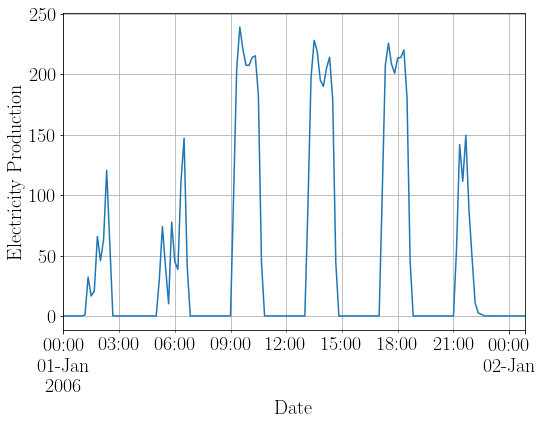
\includegraphics[width=\linewidth]{./img/solar_energy_10min_small.png}
    \caption{Solar Energy timeseries with frequency 10 min.}
    \label{fig:solar_10_min}
    \endminipage\hfill
    \minipage{0.5\textwidth}
    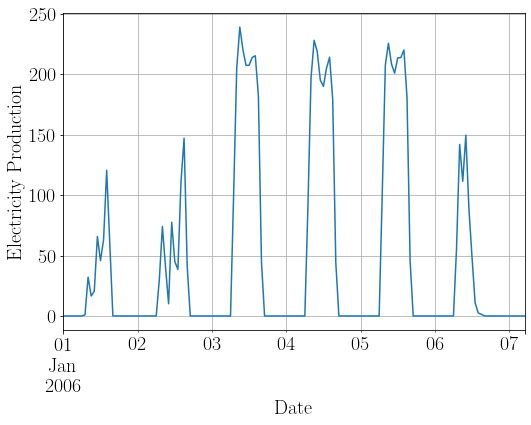
\includegraphics[width=\linewidth]{./img/solar_energy_fixed_small.png}
    \caption{Solar Energy timeseries with frequency 1 hour.}
    \label{fig:solar_fixed}
    \endminipage\hfill
\end{figure}

The S-Naive forecaster performed well on the Electricity and the M4 daily dataset with average ranks of 3.4 and 3.6 respectively. However for the Solar Energy dataset the average rank across all metrics was 8.6. This does not make sense as the solar energy dataset has the highest strength of seasonality of all datasets. Thus sampling values from previous seasons as is done in the S-Naive forecaster should bring competitive performance at least on par with the performance of S-Naive on the other datasets. After investigating this further an issue with the Solar Energy dataset in GluonTS was identified. The frequency the dataset is sampled with is 10 minutes according to the metadata. However, this could be a mistake and that the data has a frequency of 1H. In Figure \ref{fig:solar_10_min} a time series from the dataset is shown plotted using a frequency of 10 minutes. If the true frequency of the data would be 10 minutes, then the power production of the solar panels spikes for two hours and then produces zero energy for two hours. Since solar panels produce power when the sun is out during the day and not when it is night, these two hours cycles would mean that the day is two hours long. By setting the frequency to \textit{1H} instead of the original \textit{10min} the timeseries is properly aligned as in Figure \ref{fig:solar_fixed}. This is a likely cause as to why the Seasonal Naive performed poorly on the Solar Energy dataset. Since the Thetaf forecaster deseasonalizes each time series when it is run, the ranking of this could have been affected as well. The faulty frequency to the Solar Energy dataset also likely caused the automatic feature engineering in DeepAR to add calendar features to the wrong parts of the data, i.e. marking datapoints sampled in April to be sampled in December.

The second naive model, Naive2, crashed on the Electricity dataset due to it utilizing multiplicative decomposition of time series which is not suitable for time series data close to 0. The API for this model in GluonTS does not support additive decomposition, thus not much could be done to fix this. The average rank of the Naive2 method was 8.10 which makes it that fourth worst performing method of the ones tested.

The low rank of DeepFactor contradicts the results from its original paper as there, DeepFactor, outperformed DeepAR on average while in Table \ref{tab:mean_ranks} DeepAR outperforms all other algorithms. This further enforces the benefit of automatically adding exogenous variables such as calendar days and holidays to the data like DeepAR does. The original paper of DeepFactor also compares it against MQRNN and Prophet, their findings do align with the results of this comparison since DeepAR has a better average rank than both. However, Prophet did not have time to finish the benchmark on the \textit{M5} and \textit{Electricity} datasets so comparing these only by looking at the mean ranks is not fair. Comparing the mean ranks of DeepFactor and Prophet across all metrics for the Solar Energy and the M4 Daily datasets tells a similar story where DeepFactor recieves an average rank of \(10+11.5+10+9.5+9=10\) and Prophet receives the mean rank \(12+12+12+10+6.5=10.5\). Thus, for this comparison, DeepFactor is only marginally better than Prophet.

The Gaussian Process (GP) forecasting method was ranked second last, with Prophet in the last place. The GP method was suboptimally tuned as the kernel used for creating the Gaussian Processes could not be specified through the GluonTS shell when tuning. This may have led to a subpar kernel being used for the benchmark.

\begin{table}[htb]
    \centering
    \begin{tabular}{ccccccc}
        Algorithm   & \rothalf{Electricity} & \rothalf{Solar Energy} & \rothalf{M4 Daily} & \rothalf{M5} & \rothalf{Mean rank} \\
        \hline
        \multicolumn{6}{c}{\cellcolor{gray!25}MSIS}                                                                            \\
        \hline
        DeepAR      & 6.44 (1)              & 8.55 (2)               & 43.13 (2)          & 32.58 (4)    & 2.25                \\\hline
        SimpleFF    & 10.64 (3)             & 14.78 (3)              & 36.33 (1)          & 26.49 (2)    & 2.25                \\\hline
        Transformer & 6.85 (2)              & 6.41 (1)               & 49.15 (3)          & 35.38 (5)    & 2.75                \\\hline
        C-RNN       & 21.96 (4)             & 46.74 (6)              & 105.21 (4)         & 31.41 (3)    & 4.25                \\\hline
        NBEATS      & 33.35 (5)             & 46.50 (5)              & 137.24 (8)         & 57.74 (6)    & 6.00                \\\hline
        DeepFactor  & 479.13 (9)            & 53.17 (7)              & 928.47 (11)        & 20.78 (1)    & 7.00                \\\hline
        Thetaf      & 47.02 (7)             & 97.08 (11)             & 130.49 (5)         & 69.13 (7)    & 7.50                \\\hline
        S-Naive     & 35.25 (6)             & 97.07 (9)              & 131.14 (7)         & 81.28 (9)    & 7.75                \\\hline
        Prophet     & nan (10)              & 20.84 (4)              & 166.84 (9)         & nan (10)     & 8.25                \\\hline
        Naive2      & nan (10)              & 97.07 (10)             & 131.14 (6)         & 81.28 (8)    & 8.50                \\\hline
        GP          & 126.45 (8)            & 84.13 (8)              & 185.82 (10)        & nan (10)     & 9.00                \\\hline
        MQRNN       & nan (10)              & nan (12)               & nan (12)           & nan (10)     & 11.00               \\\hline
        MQCNN       & nan (10)              & nan (12)               & nan (12)           & nan (10)     & 11.00               \\\hline
    \end{tabular}
    \caption{Benchmark results with respects to the MSIS error metric. Ranks within a dataset shown in parentheses.}
    \label{tab:benchmark_results_msis}
\end{table}


\begin{table}[htb]
    \centering
    \begin{tabular}{ccccccc}
        Algorithm   & \rothalf{Electricity} & \rothalf{Solar Energy} & \rothalf{M4 Daily} & \rothalf{M5} & \rothalf{Mean rank} \\
        \hline
        \multicolumn{6}{c}{\cellcolor{gray!25}MASE}                                                                            \\
        \hline
        NBEATS      & 0.83 (3)              & 1.16 (2)               & 3.43 (4)           & 1.44 (1)     & 2.50                \\\hline
        DeepAR      & 0.75 (1)              & 1.17 (3)               & 3.81 (7)           & 1.48 (2)     & 3.25                \\\hline
        Transformer & 0.82 (2)              & 1.13 (1)               & 4.26 (8)           & 1.50 (3)     & 3.50                \\\hline
        SimpleFF    & 0.92 (5)              & 1.27 (4)               & 3.48 (5)           & 1.54 (5)     & 4.75                \\\hline
        MQCNN       & 1.22 (7)              & 1.50 (5)               & 3.51 (6)           & 1.55 (6)     & 6.00                \\\hline
        Thetaf      & 1.18 (6)              & 2.43 (11)              & 3.26 (1)           & 1.73 (8)     & 6.50                \\\hline
        S-Naive     & 0.88 (4)              & 2.43 (10)              & 3.28 (2)           & 2.03 (11)    & 6.75                \\\hline
        C-RNN       & 2.24 (8)              & 1.60 (6)               & 4.31 (9)           & 1.52 (4)     & 6.75                \\\hline
        Naive2      & nan (12)              & 2.43 (9)               & 3.28 (3)           & 2.03 (10)    & 8.50                \\\hline
        MQRNN       & 11.19 (10)            & 1.71 (7)               & 57.94 (13)         & 1.58 (7)     & 9.25                \\\hline
        DeepFactor  & 12.02 (11)            & 1.84 (8)               & 23.64 (12)         & 1.85 (9)     & 10.00               \\\hline
        GP          & 3.18 (9)              & 2.45 (12)              & 4.69 (10)          & nan (12)     & 10.75               \\\hline
        Prophet     & nan (12)              & 3.26 (13)              & 11.96 (11)         & nan (12)     & 12.00               \\\hline
        \multicolumn{6}{c}{\cellcolor{gray!25}MAPE}                                                                            \\
        \hline
        Thetaf      & 0.18 (6)              & 1.00 (1)               & 0.04 (3)           & 0.65 (1)     & 2.75                \\\hline
        S-Naive     & 0.14 (4)              & 1.00 (3)               & 0.04 (1)           & 0.88 (11)    & 4.75                \\\hline
        NBEATS      & 0.13 (3)              & 2.84 (7)               & 0.05 (5)           & 0.82 (7)     & 5.50                \\\hline
        MQCNN       & 0.22 (7)              & 2.15 (6)               & 0.05 (4)           & 0.79 (5)     & 5.50                \\\hline
        SimpleFF    & 0.14 (5)              & 2.96 (8)               & 0.05 (6)           & 0.79 (4)     & 5.75                \\\hline
        Naive2      & nan (12)              & 1.00 (2)               & 0.04 (2)           & 0.88 (10)    & 6.50                \\\hline
        DeepAR      & 0.10 (1)              & 3.29 (10)              & 0.05 (7)           & 0.87 (9)     & 6.75                \\\hline
        Transformer & 0.10 (2)              & 3.27 (9)               & 0.06 (8)           & 0.86 (8)     & 6.75                \\\hline
        C-RNN       & 0.30 (8)              & 4.92 (12)              & 0.06 (9)           & 0.79 (3)     & 8.00                \\\hline
        MQRNN       & 1.01 (11)             & 1.03 (4)               & 0.42 (13)          & 0.82 (6)     & 8.50                \\\hline
        DeepFactor  & 0.99 (10)             & 4.09 (11)              & 0.20 (12)          & 0.70 (2)     & 8.75                \\\hline
        GP          & 0.34 (9)              & 1.09 (5)               & 0.06 (10)          & nan (12)     & 9.00                \\\hline
        Prophet     & nan (12)              & 8.22 (13)              & 0.15 (11)          & nan (12)     & 12.00               \\\hline
    \end{tabular}
    \caption{Benchmark results with respect to the MASE and MAPE metrics. Ranks within a dataset shown in parentheses.}
    \label{tab:benchmark_results_MASE_MAPE}
\end{table}

% \begin{adjustbox}{center}
% <your table (i.e. the tabular or similar environment)>
% \end{adjustbox}

\begin{table}[htb]
    \centering
    \begin{tabular}{ccccccc}
        Algorithm   & \rothalf{Electricity} & \rothalf{Solar Energy} & \rothalf{M4 Daily} & \rothalf{M5} & \rothalf{Mean rank} \\
        \hline
        \multicolumn{6}{c}{\cellcolor{gray!25}Absolute Error}                                                                  \\
        \hline
        NBEATS      & 8869733 (1)           & 336976 (2)             & 11201583 (5)       & 811248 (1)   & 2.25                \\\hline
        DeepAR      & 9327671 (4)           & 339306 (3)             & 12135357 (7)       & 844784 (2)   & 4.00                \\\hline
        Transformer & 9263741 (3)           & 328560 (1)             & 13681491 (9)       & 869196 (5)   & 4.50                \\\hline
        MQCNN       & 13805770 (7)          & 432799 (5)             & 11070810 (4)       & 856588 (3)   & 4.75                \\\hline
        SimpleFF    & 9531230 (5)           & 369138 (4)             & 11234445 (6)       & 904818 (7)   & 5.50                \\\hline
        S-Naive     & 8962995 (2)           & 708874 (10)            & 10701169 (2)       & 1152816 (11) & 6.25                \\\hline
        Thetaf      & 13089580 (6)          & 708907 (11)            & 10512352 (1)       & 912691 (8)   & 6.50                \\\hline
        C-RNN       & 29287248 (8)          & 465076 (6)             & 13542748 (8)       & 861390 (4)   & 6.50                \\\hline
        Naive2      & nan (12)              & 708874 (9)             & 10701169 (3)       & 1152816 (10) & 8.50                \\\hline
        MQRNN       & 121965994 (10)        & 499512 (7)             & 205836216 (13)     & 880390 (6)   & 9.00                \\\hline
        DeepFactor  & 128561908 (11)        & 531101 (8)             & 72334786 (12)      & 1025815 (9)  & 10.00               \\\hline
        GP          & 38069033 (9)          & 715938 (12)            & 15070775 (10)      & nan (12)     & 10.75               \\\hline
        Prophet     & nan (12)              & 950621 (13)            & 40508217 (11)      & nan (12)     & 12.00               \\\hline
        \multicolumn{6}{c}{\cellcolor{gray!25}RMSE}                                                                            \\
        \hline
        DeepAR      & 1752.89 (5)           & 30.81 (3)              & 637.84 (2)         & 2.28 (2)     & 3.00                \\\hline
        NBEATS      & 1177.71 (2)           & 30.53 (2)              & 748.49 (10)        & 2.21 (1)     & 3.75                \\\hline
        Transformer & 1399.50 (4)           & 29.55 (1)              & 677.32 (5)         & 2.53 (7)     & 4.25                \\\hline
        SimpleFF    & 1229.84 (3)           & 35.58 (4)              & 672.66 (3)         & 2.79 (8)     & 4.50                \\\hline
        MQCNN       & 1850.22 (6)           & 39.29 (5)              & 672.82 (4)         & 2.31 (3)     & 4.50                \\\hline
        Thetaf      & 1936.66 (7)           & 62.51 (10)             & 630.09 (1)         & 2.43 (5)     & 5.75                \\\hline
        C-RNN       & 4629.80 (8)           & 41.28 (6)              & 745.09 (8)         & 2.39 (4)     & 6.50                \\\hline
        S-Naive     & 1139.93 (1)           & 62.52 (13)             & 705.42 (6)         & 3.30 (11)    & 7.75                \\\hline
        MQRNN       & 13405.46 (10)         & 45.92 (8)              & 5443.89 (13)       & 2.53 (6)     & 9.25                \\\hline
        DeepFactor  & 13505.91 (11)         & 42.26 (7)              & 2192.18 (12)       & 2.97 (9)     & 9.75                \\\hline
        GP          & 6113.39 (9)           & 62.52 (11)             & 747.68 (9)         & nan (12)     & 10.25               \\\hline
        Naive2      & nan (12)              & 62.52 (12)             & 705.42 (7)         & 3.30 (10)    & 10.25               \\\hline
        Prophet     & nan (12)              & 53.51 (9)              & 1464.99 (11)       & nan (12)     & 11.00               \\\hline
    \end{tabular}
    \caption{Benchmark results with respect to the Absolute Error and RMSE metrics. Ranks within a dataset shown in parentheses.}
    \label{tab:benchmark_results_abs_rmse}
\end{table}

The overall result of this empirical comparison of forecasting methods showed that DeepAR, NBEATS and the Transformer forecasting methods are the  best performing forecasting methods out of the 13 investigated. Each of these 13 models were evaluated on four complimentary datasets with diverse characteristics in terms of trend and strength and on five different metrics. Furthermore, statistical and naive models were the strongest performer for the \textit{M4 Daily} dataset but underperformed compared to DL based forecasting methods on the \textit{Solar Energy, M5} and \textit{Electricity} datasets.